\documentclass[11pt]{article}

\usepackage[margin=1.1in]{geometry}
\usepackage{amsmath,amssymb,amsthm,mathtools}
\usepackage{enumitem}
\usepackage{booktabs}
\usepackage{tikz}
\usetikzlibrary{positioning,fit,calc,arrows.meta,decorations.pathmorphing}
\usepackage[hidelinks]{hyperref}

\theoremstyle{definition}
\newtheorem{definition}{Definition}[section]
\newtheorem{construction}[definition]{Construction}
\newtheorem{example}[definition]{Example}
\newtheorem{remark}[definition]{Remark}
\newtheorem{convention}[definition]{Convention}
\newtheorem{obligation}[definition]{Obligation}

\theoremstyle{plain}
\newtheorem{theorem}[definition]{Theorem}
\newtheorem{proposition}[definition]{Proposition}
\newtheorem{lemma}[definition]{Lemma}
\newtheorem{corollary}[definition]{Corollary}

% --- notation ---
\newcommand{\sem}[1]{[\![#1]\!]}
\newcommand{\refl}[1]{\ulcorner #1 \urcorner}
\newcommand{\quo}[1]{@#1}
\newcommand{\out}[2]{#1\,!\,(#2)}
\newcommand{\for}[3]{\mathsf{for}\,(#1 \Leftarrow #2)\,\{\,#3\,\}}
\newcommand{\Let}[3]{\mathsf{let}\;#1 = #2\;\mathsf{in}\;#3}
\newcommand{\nil}{\mathbf{0}}
\newcommand{\rew}{\Rightarrow}
\newcommand{\Loc}{\Lambda}
\newcommand{\Tags}{\Sigma}
\newcommand{\Tagsb}{\Tags_{\bot}}
\newcommand{\Cfg}{\mathcal{C}}
\newcommand{\Hs}{\mathcal{H}}
\newcommand{\Hc}{\Hs_{\Cfg}}
\newcommand{\Hb}{\Hs_{B}}
\newcommand{\Jumps}{\mathcal{J}}
\newcommand{\fp}{\mathrm{fp}}
\newcommand{\PREP}{\textsc{Prepare}}
\newcommand{\SEL}{\textsc{Select}}
\newcommand{\MATCH}{\textsc{Match}}
\newcommand{\WRITE}{\textsc{Write}}
\newcommand{\id}{\mathrm{id}}
\newcommand{\bra}[1]{\langle #1 |}
\newcommand{\ket}[1]{| #1 \rangle}
\newcommand{\ketbra}[2]{| #1 \rangle\langle #2 |}
\newcommand{\cwrho}{\textsf{cwrho}}
\newcommand{\cwG}{\mathrm{cwG}}

% --- zx picture styles ---
\tikzset{
  zxz/.style={circle, draw=black, fill=green!25, minimum size=5.5mm, inner sep=0pt, font=\scriptsize},
  zxx/.style={circle, draw=black, fill=red!30,   minimum size=5.5mm, inner sep=0pt, font=\scriptsize},
  zxh/.style={rectangle, draw=black, fill=yellow!45, minimum size=4mm, inner sep=1pt, font=\scriptsize},
  zxbox/.style={rectangle, draw=black, fill=blue!8, minimum height=9mm, inner sep=3pt, font=\small},
  zxw/.style={draw=black, line width=0.4pt}
}

\title{\bfseries Complex-Weighted Rho to ZX\\[2pt]
\large Compiling weighted graph-structured lambda theories to the ZX-calculus\\
by symbolic execution}
\author{L.\,G.~Meredith\\\small F1R3FLY.io}
\date{\today}

\begin{document}
\maketitle

\begin{abstract}
The quantum reading of a weighted graph-structured lambda theory (GSLT) has until now been
built as the stochastic reading with $\mathbb{R}_{\geq 0}$ replaced by $\mathbb{C}$. That
construction leaves phase with nowhere to live: amplitude is made to do the work of a rate,
the classical marginal is recovered only by choosing a normalisation, and no interference at
the level of rewriting survives. We take a different target. Given a complex-weighted GSLT
$\cwG$, we compile a program to an expression in the ZX-calculus by symbolically executing it
against a cost budget. Every GSLT desugars into the rho calculus by a location-indexed
installation whose location channels are injective; we use that factorisation, so only one
compiler is written, from complex-weighted rho ($\cwrho$) to ZX. Configurations are functions
from locations to head tags, so the state space is a tensor product indexed by locations and
the independence structure of the calculus is the tensor structure of the diagram; parallel
composition is not needed and is not assumed. A rewrite instance becomes a scalar times a
matrix unit on its footprint, which in ZX is a pair of disconnected spiders. One step is a
block encoding: a branch register indexed by \emph{all} jumps of the budgeted address space,
a \PREP\ stage whose amplitudes \emph{are} the weight map, and a \SEL\ stage of controlled
matrix units. The principal observation is that the stochastic and the quantum semantics are
the same diagram with different caps on the branch wire: measuring the branch register in the
$Z$ basis reproduces the selection step of the stochastic simulation algorithm with rates
$|w|^2$, while measuring it in the $X$ basis --- post-selecting the $\ket{+}$ outcome ---
performs the coherent sum over derivations. Interference is therefore effected by projection,
not by unitary erasure: we prove that a retained branch record is a which-path record and
suppresses interference exactly, so measurement is not a fallback for non-unitarity but the
engine of coherence. We give the conditions under which a step dilates to an isometry
(a per-configuration normalisation of $|w|^2$, made total by fictitious jumps at normal
forms) and hence stands a chance of circuit extraction, and we record what is merely
simulable otherwise. A worked example is computed, not asserted: a two-spike, two-neuron
network in which two weight maps of identical magnitude are indistinguishable
under the $Z$ cap and, under the $X$ cap, differ between never co-firing and
co-firing two times in three. Spatial-behavioural key formulae compile to phase
gadgets controlled on the subsystem that decides them, so the partition discipline of the weighted-GSLT note is
exactly the condition that the \PREP\ diagonal is single-valued, and the requirement that
keys be structural is exactly the condition that the gadgets have bounded arity.
\end{abstract}

\tableofcontents

\section{Introduction}\label{sec:intro}

\subsection{The diagnosis}

In the weighted-GSLT note~\cite{weighted} a finitely presentable GSLT is equipped with a
weight map: rewrite rules carry weights, keys are spatial-behavioural formulae refining the
left-hand side, and a map instance is part of a state specification, so that weights may
change as the system runs. With weights in $\mathbb{R}_{\geq 0}$ the story is settled: the
weights are propensities, redex multiplicity is Gillespie's $h$, and the simulator samples a
continuous-time Markov chain.

With weights in $\mathbb{C}$ the story was built by analogy, and the analogy does not hold.
The difficulty is visible in the one place where the two constructions had to be reconciled:
if $m$ derivations lead to the same target, is the matrix element $\sum_i \sqrt{\lambda_i}$
or $\sqrt{\sum_i \lambda_i}$? The second was chosen, on the correct grounds that only it is a
conservative lift of the classical semantics; but the choice was forced precisely because the
construction had no way to keep the $m$ derivations apart, and paying for conservativity in
that coin buys a codomain in which no rewrite-level interference is possible at all. What was
supposed to be the quantum theory became the classical theory with a decorative phase, and
the note recorded the residue as an open thread: per-derivation amplitudes require a codomain
indexed by derivations, which is a different paper.

This is that paper, and the resolution is not a better normalisation convention. It is a
different target.

\subsection{What changes}

Three moves.

\paragraph{Factor through rho.} Every finitely presentable GSLT desugars into the rho
calculus by the location-indexed installation of~\cite[\S4.2, App.~A]{knotted}. A base rewrite
is installed at \emph{every} location whose head matches, so no reduction strategy is imposed;
the channel of a location is its reflection, $c(\ell) = @\ell$, which is injective; and
the operational-correspondence proposition gives a step-for-step bisimulation in which each
firing at $\ell$ is a transition labelled $c(\ell)$. Consequently the context-labelled
transition labels \emph{are} derivation identities. The codomain indexed by derivations that
the earlier note deferred is already present in the rho image, for free. We therefore write one
compiler, from $\cwrho$ to ZX, and inherit the rest.

\paragraph{Make configurations the state and listeners the program.} Under the desugaring a
term is a parallel composition of messages $\out{c(\ell)}{\underline{f}}$, one per node,
publishing that node's head tag at that node's location channel. The dynamic content of a
running program is therefore a function from locations to head tags. This is a tensor product
indexed by locations. Crucially it requires no parallel composition operator in the source:
lambda, SKI and Turing machines have GSLT presentations and none of them has one, but all of
them have locations, because every GSLT has one-hole contexts by construction. The tensor
structure of the ZX diagram tracks the independence relation on redexes; parallel composition,
where a calculus has it, merely makes that relation syntactically manifest.

\paragraph{Let phase live in the branch register.} A single step is a sum over enabled jumps,
and the ZX-calculus has composition and tensor but no primitive for linear combination. We
realise the sum as a block encoding with an explicit branch register $B$ indexed by all jumps
of the budgeted address space. The weight map becomes the amplitudes of the \PREP\ state on
$B$. That is where phase lives, and it is where it does work: the branch wire is where
derivations meet.

\subsection{The principal observation}

Once the diagram is built, the classical and the quantum readings are not two constructions
but two ways of capping one wire.

\begin{quote}
\emph{Measure the branch register in the $Z$ basis and you have the selection step of the
stochastic simulation algorithm, with the jump chosen with probability proportional to
$|w|^2$. Measure it in the $X$ basis, keeping the $\ket{+}$ outcome, and you have the coherent
sum over derivations, with the weights' relative phases doing exactly what phases do.}
\end{quote}

In ZX these two are the same diagram with a green cap or a red cap on one wire. Theorems~
\ref{thm:classical} and~\ref{thm:coherent} make this precise. Theorem~\ref{thm:whichpath}
explains why there is no third option: a retained branch record is a which-path record, and a
unitary cannot erase one, so coherent recombination of distinct derivations is achieved by
projection and by nothing else. Measurement is not the fallback for programs that fail to be
unitary; it is the mechanism of interference.

\subsection{Contributions}

\begin{enumerate}[leftmargin=*]
  \item A configuration space for $\cwrho$ forced by the desugaring rather than chosen: a
        qudit per location, of dimension one more than the number of constructors
        (\S\ref{sec:config}). Structural congruence is quotiented by construction
        (Proposition~\ref{prop:acfree}) and the installed listeners are invariant, hence
        compile to the diagram rather than to the state (Proposition~\ref{prop:listener}).
  \item Rewrite instances as scalar multiples of matrix units on footprints, with disjoint
        footprints tensoring (\S\ref{sec:matrixunits}, Proposition~\ref{prop:independence}).
  \item The one-step block encoding $V = \sum_j \ket{j}_B \otimes K_j$ and its ZX realisation
        (\S\ref{sec:zx}), with the weight map appearing as the \PREP\ amplitudes and
        spatial-behavioural key formulae as phase gadgets controlled on the subsystem that
        decides them (\S\ref{ssec:keys}).
  \item The symbolic execution algorithm, its termination by cost budget, and the computation
        of the address set (\S\ref{sec:symbolic}).
  \item The two caps and their theorems: $Z$-basis measurement recovers the SSA selection step
        with rates $|w|^2$ (Theorem~\ref{thm:classical}); $X$-basis post-selection performs the
        coherent sum (Theorem~\ref{thm:coherent}); no unitary interpolates
        (Theorem~\ref{thm:whichpath}) (\S\ref{sec:caps}).
  \item A dilation theorem: a uniformised weight map, made total by fictitious jumps at normal
        forms, yields an isometry and hence a unitary extension
        (\S\ref{sec:unitary}, Theorem~\ref{thm:dilation}).
  \item A worked example, computed rather than asserted (\S\ref{sec:network}):
        a coherent spiking network whose two weight maps have identical
        magnitudes, hence identical stochastic behaviour, and whose coherent
        behaviour differs completely --- co-firing probability $0$ against
        $2/3$. And a plasticity result: a synapse-specific Hebbian read
        destroys exactly the coherence that produced the correlation, at the
        rate $\eta^2/(1+\eta^2)$ (Proposition~\ref{prop:exchange}), while a
        read of either index alone costs nothing (Lemma~\ref{lem:coarse}).
  \item A revision of the multiplicity question. The location encoding makes $m$ ``indistinguishable''
        derivations genuinely distinct branches, so $m$ and $m^2$ are the correct classical and
        coherent answers respectively, and neither is an artefact (Remark~\ref{rem:mult}).
\end{enumerate}

\subsection{What this note does not do}

It does not settle the elaboration of MeTTaIL tuple-pattern receives into core rho. Both source
papers treat that elaboration as unnecessary detail~\cite[\S2.2]{optimal}; we work at the
granularity of the context-labelled transition system, where one rule firing is one labelled
transition, and record the residual obligation in \S\ref{sec:open}. It does not give a
qudit-native ZX treatment: we compile to qubits because the tooling does. It does not claim
that any interesting program is extractable to hardware today; \S\ref{sec:unitary} states what
would have to hold.

\section{Complex-weighted rho}\label{sec:cwrho}

\subsection{The desugaring, recalled}

We recall only what is needed. Fix a finitely presentable GSLT $G$ with constructor signature
$\Tags$ (each $f \in \Tags$ of arity $\mathrm{ar}(f)$) and rewrite rules $\mathcal{R}$.

\begin{definition}[Locations and location channels~{\cite[Def.~4.3]{knotted}}]\label{def:loc}
A \emph{location} is a finite path $\ell = \langle (f_1,i_1),\dots,(f_m,i_m)\rangle$ from the
root of a term, where $(f,i)$ descends into the $i$-th argument of an $f$-node; $\varepsilon$
is the root and $\ell\cdot(f,i)$ the child. The location channel is $c(\ell) := @\ell$.
The map $c$ is injective.
\end{definition}

\begin{definition}[The desugaring~{\cite[App.~A]{knotted}}]\label{def:desugar}
For a constructor $f$ of arity $n$,
\[
  \sem{f(t_1,\dots,t_n)}_\ell \;=\; \out{c(\ell)}{\underline{f}}
  \ \big|\ \textstyle\bigm|_{i=1}^{n} \sem{t_i}_{\ell\cdot(f,i)},
\]
and for a base rewrite $L \rew R$ with $\mathrm{hd}(L) = f$,
\[
  \sem{L \rew R} \;=\; \textstyle\bigm|_{\ell\,:\,\mathrm{hd}=f}\
  \for{\sem{L}}{c(\ell)}{\ \out{c(\ell)}{\sem{R}_\ell}\ \big|\ \sem{L \rew R}\ },
\]
the inner copy re-installing the listener after each fire by the reflection idiom, with no
replication. A whole GSLT is $\sem{G} = \bigm|_{(L\rew R)\in\mathcal{R}} \sem{L\rew R}$, with
equations compiled to structural congruence. A term $t$ is run by injecting
$\sem{t}_\varepsilon$ on a fresh root.
\end{definition}

Two features of this presentation do the work of this note.

\begin{proposition}[Firings are labelled by locations]\label{prop:labels}
Each base-rewrite firing of $t$ at location $\ell$ corresponds to a transition of $\sem{t}$
labelled $c(\ell)$, and conversely; and since $c$ is injective, distinct firings carry distinct
labels.
\end{proposition}

\begin{proof}
The correspondence is~\cite[Prop.~4.5]{knotted}. Distinctness is injectivity of $c$
(Definition~\ref{def:loc}).
\end{proof}

\begin{proposition}[No strategy is imposed]\label{prop:nostrategy}
The compiled program admits a firing at every location whose head matches a rule's left-hand
side.
\end{proposition}

\begin{proof}
Immediate from the indexed parallel composition $\bigm|_{\ell : \mathrm{hd}=f}$ in
Definition~\ref{def:desugar}.
\end{proof}

Proposition~\ref{prop:nostrategy} is worth dwelling on, because the worked example of the
companion paper~\cite[\S5.1]{optimal} compiles the lambda calculus under weak head reduction
and it is easy to read the restriction as belonging to the translation. It does not: the
restriction is carried by the source presentation, in the contextual rule
$M \rew M' \Rightarrow \mathit{app}(M,N)\rew\mathit{app}(M',N)$, which is what encodes weak head
reduction. Present lambda with contextual rules at every position and the compiled program has
every $\beta$-redex live. This matters here more than it does classically: as
\S\ref{sec:whichpath} shows, the interference in a confluent calculus lives precisely in the
multiplicity of derivations that a strategy would have suppressed.

\subsection{Weights}

\begin{definition}[Complex-weighted GSLT]\label{def:cwg}
A \emph{complex-weighted GSLT} $\cwG = (G, \mathcal{K}, w)$ consists of a finitely presentable
GSLT $G$; for each rule $r \in \mathcal{R}$ a finite set $\mathcal{K}_r$ of \emph{keys}, which
are structural formulae of the OSLF-generated logic of $G$ refining the left-hand side of $r$
and forming a partition of it; and a weight map
\[
  w \;:\; \Cfg \times \mathcal{R} \times \textstyle\bigcup_r \mathcal{K}_r \longrightarrow \mathbb{C},
\]
where $\Cfg$ is the set of configurations (Definition~\ref{def:cfg}). The dependence on the
first argument is what makes the map dynamic --- the distinguishing feature of the framework
of~\cite{weighted} relative to SPiM --- and, as \S\ref{ssec:keys} shows, it is also what makes
the map a controlled gadget rather than a constant.
\end{definition}

We carry forward two requirements from~\cite{weighted} without re-arguing them, and observe in
\S\ref{ssec:keys} that each has an exact ZX-side meaning.

\begin{convention}[Partition]\label{conv:partition}
For each rule $r$, the keys $\mathcal{K}_r$ partition the refinement lattice below the
left-hand side of $r$, with a default class completing the partition.
\end{convention}

\begin{convention}[R3: keys are structural]\label{conv:r3}
Keys are drawn from the structural fragment of the generated logic --- one connective per term
former, plus $\wedge$, $\top$ and the complement needed for the default class. Modal keys
($\langle K \rangle$, $[K]$, $\nu$) are refused at elaboration time.
\end{convention}

\begin{remark}[Where the codomain restriction goes]\label{rem:codomain}
The earlier note removed the $|z| \le 1$ clamp and interpreted a complex weight through
$\lambda(z) = |z|^2$. Both survive here, but they are no longer the whole story: $|w|^2$ is
what the $Z$-cap sees (Theorem~\ref{thm:classical}) and $\arg w$ is what the $X$-cap sees
(Theorem~\ref{thm:coherent}). The interpretation map $\lambda$ is the shadow the classical
reading casts, not a definition of the quantum one.
\end{remark}

\subsection{Fictitious jumps}\label{ssec:fictitious}

The generator convention of~\cite{weighted} skips self-transitions when forming the diagonal
and treats them as fictitious jumps. We adopt the mirror-image convention, for a reason that
becomes a theorem in \S\ref{sec:unitary}.

\begin{convention}[Identity jump]\label{conv:idjump}
Every configuration carries an additional jump $\iota$ with $K_\iota = w_\iota \cdot \id$,
enabled exactly when no other jump is enabled. Normal forms therefore have a nonempty enabled
set.
\end{convention}

Without Convention~\ref{conv:idjump} the block encoding of \S\ref{sec:zx} annihilates normal
forms, the total weight out of a normal form is zero, and the normalisation condition of
Theorem~\ref{thm:dilation} cannot hold anywhere the computation actually stops. With it, a
normal form is a fixed point of the step map and the theory is total.

\section{The configuration space}\label{sec:config}

\subsection{Configurations}

\begin{definition}[Configuration]\label{def:cfg}
Let $\Loc$ be a finite set of locations (the \emph{address set}; \S\ref{ssec:address} computes
it) and $\Tagsb = \Tags \sqcup \{\bot\}$. A \emph{configuration} is a function
$\gamma : \Loc \to \Tagsb$, where $\gamma(\ell) = f$ means the message
$\out{c(\ell)}{\underline{f}}$ is present and $\gamma(\ell) = \bot$ means no message is present
at $\ell$. Write $\Cfg = \Tagsb^{\Loc}$.
\end{definition}

\begin{proposition}[Structural congruence is free]\label{prop:acfree}
The associativity, commutativity and unit laws of parallel composition are quotiented by
Definition~\ref{def:cfg} without any equational machinery in the target.
\end{proposition}

\begin{proof}
A configuration is a function on locations, not a sequence or multiset of processes. The
desugaring publishes exactly one head tag per location, so the parallel composition of the
messages of a term is recovered from $\gamma$ up to $\equiv$, and any two $\equiv$-equivalent
message assemblies give the same $\gamma$.
\end{proof}

This is the ZX-side counterpart of the source-side fact that equations compile to structural
congruence and are ``colour-respecting, cost-free, \emph{iso} in the target rather than
motion''~\cite[\S4.2]{knotted}: equations of the presented GSLT generate no diagram content
whatsoever. The slogan of~\cite{weighted} --- that a weighted GSLT is quantum exactly to the
extent that its presentation withholds equations from the quotient --- acquires a sharp
operational form here: what is withheld from the quotient is what gets a wire.

\begin{proposition}[Listeners are static]\label{prop:listener}
The multiset of installed listeners is invariant under reduction.
\end{proposition}

\begin{proof}
By Definition~\ref{def:desugar} the continuation of a firing is
$\out{c(\ell)}{\sem{R}_\ell} \mid \sem{L \rew R}$, whose second component re-installs the
entire indexed family. Hence after any firing the installed family is again $\sem{G}$.
\end{proof}

Proposition~\ref{prop:listener} is what makes the state space small. Listeners are the program;
they compile to the \emph{diagram}. Messages are the state; they compile to the \emph{wires}.
Nothing about the listener structure needs to be represented in the Hilbert space.

\subsection{The Hilbert space}

\begin{definition}[State space]\label{def:hilbert}
$\Hc := \bigotimes_{\ell \in \Loc} \mathbb{C}^{\Tagsb}$, with computational basis
$\{\ket{\gamma} : \gamma \in \Cfg\}$ and $\ket{\gamma} = \bigotimes_{\ell} \ket{\gamma(\ell)}$.
\end{definition}

Three things are worth saying about this definition, because it is the one place where the
whole design is decided.

\begin{remark}[The tensor structure is the independence structure]\label{rem:independence}
The factorisation of $\Hc$ is indexed by locations, and locations are what every GSLT has. Two
rewrite instances at locations that are not prefix-comparable act on disjoint tensor factors
and commute. In a calculus with parallel composition, top-level parallel components are exactly
the incomparable locations below the root, so the familiar reading of $\mid$ as tensor is
recovered as a special case; in lambda or SKI, where disjointness of redexes is a theorem about
residuals rather than a syntactic given, the same tensor decomposition is available because the
same locations are.
\end{remark}

\begin{remark}[Contrast with $\ell^2(\mathrm{Terms}/\!\equiv)$]\label{rem:contrast}
The quantum section of~\cite{weighted} takes the state space to be $\ell^2$ of the reachable
configurations, indexed by configuration keys. That is correct and it is the right choice for a
simulator that owns its own state graph. It is the wrong choice here: an unstructured index set
produces a dense operator with no tensor locality, and every rewrite rule of the ZX-calculus is
local. A compiler that emitted such an operator would have drawn its matrix as a diagram and
gained nothing. Definition~\ref{def:hilbert} exists to be factorised.
\end{remark}

\begin{remark}[Qudits]\label{rem:qudits}
$\dim \mathbb{C}^{\Tagsb} = |\Tags| + 1$. We treat the qudit picture as primitive because it is
the one the calculus dictates, and compile to qubits in \S\ref{ssec:qubits} because the tooling
is qubit-native. A qudit-native ZX variant would remove that compilation step.
\end{remark}

\subsection{The budget and the address set}\label{ssec:address}

The desugaring installs listeners at every location whose head matches, and the set of such
locations is not \emph{a priori} finite: a right-hand side may be larger than the left, and
recursion, reached in rho through reflection rather than through a primitive replication, is a
non-well-founded inhabitant of the process object. The risk ledger of~\cite{knotted} prices
this exactly: a finitely presentable GSLT with finite synchronisation trees is hereditarily
finite and commits no infinite risk, while recursion costs one $\omega$. The budget is what
keeps the compiler inside the finitary core.

\begin{definition}[Budget and address set]\label{def:budget}
Let $\beta \in \mathbb{N}$ be a \emph{step budget} and $t$ the initial term. The
\emph{address set} $\Loc_\beta(t)$ is the set of locations occurring in any term reachable from
$t$ in at most $\beta$ firings. The \emph{jump set} $\Jumps_\beta(t)$ is the set of triples
$j = (r, \ell, \kappa)$ with $r \in \mathcal{R}$, $\ell \in \Loc_\beta(t)$ a location where
$\mathrm{hd}(L_r)$ could sit, and $\kappa \in \mathcal{K}_r$, together with the identity jump
$\iota$.
\end{definition}

We compute $\Loc_\beta(t)$ by symbolic execution (\S\ref{sec:symbolic}); it is not assumed.

\begin{proposition}[Width bound]\label{prop:width}
$|\Loc_\beta(t)| \le |\Loc(t)| \cdot g^\beta$ where $g$ is the maximum, over rules
$L \rew R$, of the number of locations of $R$ divided by the number of locations of $L$
consumed. Consequently $\dim \Hc \le (|\Tags|+1)^{|\Loc(t)|\,g^\beta}$.
\end{proposition}

\begin{proof}
Each firing replaces the sub-term at its location by the right-hand side, whose location count
is bounded by $g$ times that of the left; iterate $\beta$ times.
\end{proof}

The bound is honest rather than useful when $g > 1$, and it is the principal practical limit on
this compiler. For calculi where a step does not grow the term --- Turing machines, and
lambda under a linear discipline --- $g = 1$ and the width is fixed by the initial term. For
$\beta$-reduction with duplication, $g > 1$ and the width grows geometrically in the budget.
We return to this in \S\ref{ssec:sparsity}.

\section{Rewrites as matrix units}\label{sec:matrixunits}

\subsection{Footprints}

\begin{definition}[Footprint]\label{def:footprint}
Let $j = (r,\ell,\kappa) \in \Jumps_\beta(t)$ with $r : L \rew R$. The \emph{read set}
$\mathrm{rd}(j) \subseteq \Loc$ is the set of locations of $\ell \cdot \mathrm{dom}(L)$
inspected by the pattern $L$ together with those inspected by the key $\kappa$; the
\emph{write set} $\mathrm{wr}(j)$ is $\ell \cdot \mathrm{dom}(R)$ together with those locations
of $\ell\cdot\mathrm{dom}(L)$ vacated by the rewrite. The \emph{footprint} is
$\fp(j) = \mathrm{rd}(j)\cup\mathrm{wr}(j)$.
\end{definition}

\begin{remark}[Why $\kappa$ enters the read set]\label{rem:kapparead}
Convention~\ref{conv:r3} is doing work here. A structural key is a formula built from one
connective per term former, so satisfaction of $\kappa$ is decided by inspecting finitely many
locations at bounded depth below $\ell$; the depth grading $d(\varphi)$ of~\cite{weighted}
bounds it. A modal key would not have this property --- $\langle K \rangle\varphi$ asks about
the transition relation, not about the configuration --- and its read set would not be a finite
set of locations at all. R3 is therefore not merely a hygiene requirement inherited from a
referee; it is the condition under which a footprint exists.
\end{remark}

\subsection{The elementary operator}

Write $\pi_S : \Cfg \to \Tagsb^{S}$ for restriction to $S \subseteq \Loc$, and for a pattern
$P$ at $\ell$ write $\hat{P}_\ell \in \Tagsb^{\mathrm{dom}}$ for the tag assignment it demands.

\begin{definition}[Elementary operator]\label{def:K}
For $j = (r,\ell,\kappa)$ with $r : L \rew R$, and a configuration argument $\gamma$,
\[
  K_j \;=\; \ketbra{\hat{R}_\ell}{\hat{L}_\ell}_{\fp(j)} \otimes \id_{\Loc \setminus \fp(j)},
\]
a \emph{matrix unit} on the footprint. The weight is not carried by $K_j$; it is carried by the
branch register (\S\ref{ssec:prepare}).
\end{definition}

Note that $K_j$ is defined for every $j \in \Jumps_\beta(t)$, whether or not $j$ is enabled at a
given configuration: if $\gamma$ does not match $\hat{L}_\ell$ then $K_j\ket{\gamma} = 0$.
Enabledness is therefore not a side condition to be checked before building the diagram; it is
the vanishing of a term in it. This is what allows the branch register to be indexed by the
whole jump set, independently of the configuration --- a point we return to in
Remark~\ref{rem:allj}.

\begin{proposition}[Correctness of the elementary operator]\label{prop:Kcorrect}
For $\gamma \in \Cfg$, $K_j \ket{\gamma} = \ket{\gamma'}$ if the firing of $r$ at $\ell$ in
refinement class $\kappa$ is enabled at $\gamma$ and yields $\gamma'$, and $K_j\ket{\gamma} = 0$
otherwise.
\end{proposition}

\begin{proof}
$\ketbra{\hat{R}_\ell}{\hat{L}_\ell}$ acts as the identity outside $\fp(j)$ and, on $\fp(j)$,
sends the pattern $\hat{L}_\ell$ to $\hat{R}_\ell$ and every other assignment to $0$. Matching
$\hat{L}_\ell$ on $\mathrm{rd}(j)$ is, by Definition~\ref{def:footprint} and
Remark~\ref{rem:kapparead}, exactly the conjunction of the pattern match of $L$ and satisfaction
of $\kappa$; by Convention~\ref{conv:partition} exactly one $\kappa$ per $(r,\ell)$ can match.
The resulting configuration is $\gamma$ with $\fp(j)$ overwritten by $\hat{R}_\ell$, which is
the desugared image of the rewritten term by Definition~\ref{def:desugar}.
\end{proof}

\begin{proposition}[Independence tensors]\label{prop:independence}
If $\fp(j) \cap \fp(j') = \emptyset$ then $K_j K_{j'} = K_{j'} K_j$, and
$K_j K_{j'} = (\ketbra{\hat{R}}{\hat{L}}_{\fp(j)} \otimes \ketbra{\hat{R}'}{\hat{L}'}_{\fp(j')})
\otimes \id$.
\end{proposition}

\begin{proof}
Operators acting on disjoint tensor factors, extended by the identity elsewhere, commute and
their product is the tensor of their non-trivial parts.
\end{proof}

Proposition~\ref{prop:independence} is the formal content of Remark~\ref{rem:independence}: the
independence relation on redexes is disjointness of footprints, which is decided by
prefix-incomparability of locations plus the bounded depth of the patterns and keys. It is
available in every GSLT, and no parallel composition operator is required to state it.

\begin{proposition}[Rank]\label{prop:rank}
$\mathrm{rank}(K_j) = (|\Tags|+1)^{|\Loc| - |\fp(j)|}$; in particular $K_j$ is not unitary
unless $\fp(j) = \emptyset$.
\end{proposition}

\begin{proof}
A matrix unit on $\fp(j)$ has rank one; tensoring with the identity on the complement multiplies
the rank by the dimension of the complement. A unitary on $\Hc$ has full rank
$(|\Tags|+1)^{|\Loc|}$.
\end{proof}

Proposition~\ref{prop:rank} is the reason this note takes the position it does about
measurement. Non-unitarity is not an unfortunate property of badly-behaved weight maps; it is
present in the very first operator we write down, for the structural reason that a rewrite
destroys information about which redex fired. The ZX-calculus is indifferent --- its diagrams
denote arbitrary linear maps --- and \S\ref{sec:unitary} says exactly what has to be added back
to recover a unitary.

\section{The ZX realisation}\label{sec:zx}

\subsection{Qudits to qubits}\label{ssec:qubits}

Fix $q = \lceil \log_2 (|\Tags|+1)\rceil$ and an injection
$\mathrm{enc} : \Tagsb \hookrightarrow \{0,1\}^q$ with $\mathrm{enc}(\bot) = 0^q$. Each location
becomes a $q$-qubit register; $\Hc$ becomes $(\mathbb{C}^2)^{\otimes q|\Loc|}$. Pattern matching
becomes comparison against a constant bit string, and tag writing becomes assignment of a
constant bit string, both on $q$ qubits.

\begin{remark}
The encoding is not canonical and the choice matters for diagram size. Assigning
$\mathrm{enc}(\bot) = 0^q$ means an empty location is the all-zero register, so the vast
majority of the diagram's inputs are $\ket{0}$, which ZX simplifiers exploit aggressively. A
Gray-coded assignment of the remaining tags, ordering by arity, further reduces the Toffoli
depth of the match predicates of \S\ref{ssec:predperm}. We do not optimise here.
\end{remark}

\subsection{Matrix units are disconnected spiders}

\begin{lemma}[Matrix unit]\label{lem:matrixunit}
For $a,b \in \{0,1\}$, the map $\ketbra{b}{a}$ on one qubit is, up to a scalar, the ZX diagram
consisting of two disconnected one-legged $X$-spiders: an effect of phase $a\pi$ on the input
wire and a state of phase $b\pi$ on the output wire. For bit strings, tensor componentwise.
\end{lemma}

\begin{proof}
The one-legged $X$-spider with phase $0$ is $\ket{+}$ up to scalar; with phase $\pi$ it is
$\ket{-}$. Their $Z$-basis counterparts are the one-legged $Z$-spiders. Taking the $X$-spider
of phase $a\pi$ as an effect gives $\bra{a}$ up to scalar in the appropriate colour convention,
and as a state gives $\ket{b}$; a disconnected state-effect pair denotes the outer product.
\end{proof}

\begin{center}
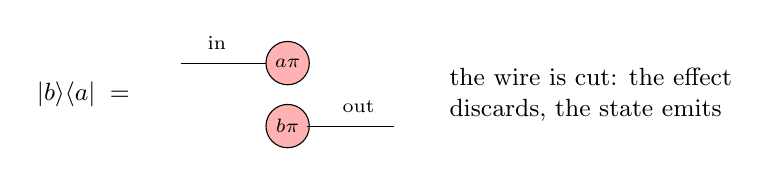
\begin{tikzpicture}[baseline]
  \node[font=\small] at (-1.0,0.35) {$\ketbra{b}{a} \;=\;$};
  \draw[zxw] (0.2,0.75) -- (1.3,0.75);
  \node[zxx] (e) at (1.55,0.75) {$a\pi$};
  \node[zxx] (s) at (1.55,-0.05) {$b\pi$};
  \draw[zxw] (1.8,-0.05) -- (2.9,-0.05);
  \node[font=\scriptsize] at (0.65,1.0) {in};
  \node[font=\scriptsize] at (2.45,0.2) {out};
  \node[font=\small, align=left] at (5.4,0.35) {the wire is cut: the effect\\ discards, the state emits};
\end{tikzpicture}
\end{center}

The picture makes the semantics vivid: the wire is \emph{cut}. Everything the input said about
this qubit is discarded and a constant is emitted. That is what a rewrite does to its footprint,
and it is why a step is not invertible.

\subsection{\PREP: the weight map is a state}\label{ssec:prepare}

Let $N = |\Jumps_\beta(t)|$ and let $B$ be a register of $b = \lceil \log_2 N\rceil$ qubits with
basis $\{\ket{j} : j \in \Jumps_\beta(t)\}$.

\begin{definition}[\PREP]\label{def:prepare}
For a configuration argument $\gamma$, the \PREP\ state is
\[
  \ket{\mathrm{prep}(\gamma)} \;=\; \sum_{j \in \Jumps_\beta(t)} w(\gamma, j)\,\ket{j} \;\in\; \Hb .
\]
\end{definition}

This is the note's central relocation. In~\cite{weighted} the weight enters as a coefficient of
a jump operator; here it enters as an amplitude of a state on a register whose basis indexes
jumps. The consequences are immediate and are worth listing.

\begin{enumerate}[leftmargin=*]
  \item \emph{Phase has somewhere to live.} $\arg w(\gamma,j)$ is a relative phase between basis
        vectors of $\Hb$, and relative phases between basis vectors of a register that is later
        recombined are exactly what interferes.
  \item \emph{Uniform magnitudes make \PREP\ unitary.} If $|w(\gamma,j)|$ is independent of $j$
        then $\ket{\mathrm{prep}(\gamma)} = D(\gamma)\ket{+}^{\otimes b}$ up to scalar, where
        $D(\gamma) = \sum_j e^{i\arg w(\gamma,j)}\ketbra{j}{j}$ is a diagonal unitary; in ZX,
        $\ket{+}^{\otimes b}$ is $b$ one-legged $X$-spiders of phase $0$, and $D$ is a family of
        phase gadgets.
  \item \emph{Non-uniform magnitudes are the only source of non-unitarity in \PREP,} and they are
        handled by the same post-selection that handles everything else
        (\S\ref{ssec:onestep}).
  \item \emph{The partition discipline is what makes $D$ single-valued.} Convention~\ref{conv:partition}
        says exactly one key per $(r,\ell)$ matches at a given $\gamma$, so
        $w(\gamma,\cdot)$ is a function, so $D(\gamma)$ is a diagonal operator rather than a
        relation.
\end{enumerate}

\begin{remark}[Why $B$ indexes all jumps, not the enabled ones]\label{rem:allj}
Indexing $B$ by the enabled jumps at $\gamma$ would make the register's dimension
state-dependent, which is not a thing a wire can be. Because $K_j$ annihilates configurations at
which $j$ is disabled (Proposition~\ref{prop:Kcorrect}), we may index $B$ by the whole of
$\Jumps_\beta(t)$ and let the disabled branches contribute zero. The price is width, $b = \lceil
\log_2 N\rceil$ qubits per step; the benefit is that the diagram is configuration-independent,
which is what makes it a \emph{compiled} object rather than a trace.
\end{remark}

\subsection{Key formulae are phase gadgets}\label{ssec:keys}

$D(\gamma)$ depends on $\gamma$, so it is not a constant diagonal but a controlled one. Its
realisation is where the spatial-behavioural logic enters the diagram.

\begin{construction}[Key gadget]\label{con:keygadget}
Let $j = (r,\ell,\kappa)$. By Convention~\ref{conv:r3} and Remark~\ref{rem:kapparead}, $\kappa$
is a structural formula whose satisfaction at $\gamma$ is a Boolean function of
$\pi_{\mathrm{rd}(j)}(\gamma)$. Compile that Boolean function to a reversible circuit
$\MATCH_j$ writing a flag qubit $f_j$; then apply, controlled on $f_j$ and on $B = j$, the phase
$e^{i\arg w(\gamma,j)}$, which is a $Z$-spider phase on the $B$ register conjugated by the
control. The magnitude $|w(\gamma,j)|$, if not uniform, is applied as a non-unitary diagonal by
the same control and absorbed into the post-selection budget.
\end{construction}

\begin{proposition}[Gadget arity]\label{prop:arity}
The gadget of Construction~\ref{con:keygadget} touches $q\cdot|\mathrm{rd}(j)| + b + 1$ qubits,
and $|\mathrm{rd}(j)|$ is bounded by the number of locations at depth at most
$d(\kappa) + \mathrm{depth}(L_r)$ below $\ell$.
\end{proposition}

\begin{proof}
The read set is determined by the pattern and the key; the depth grading of~\cite[\S3]{weighted}
bounds the key's reach, and the left-hand side's depth bounds the pattern's.
\end{proof}

Proposition~\ref{prop:arity} is the payoff of R3 in its second guise. Locality of a key formula
--- which locations it mentions --- becomes locality of the gadget --- which wires it touches ---
which becomes tractability of simplification, since every rewrite rule of the ZX-calculus is
local. A logic fragment is affordable here exactly when its formulae are decided by a
bounded-arity gadget, which gives a non-arbitrary criterion for the ideal-versus-checkable split
that~\cite{weighted} states methodologically.

\subsection{\SEL\ and the one-step diagram}\label{ssec:onestep}

\begin{definition}[\SEL]\label{def:select}
$\SEL := \sum_{j \in \Jumps_\beta(t)} \ketbra{j}{j}_B \otimes K_j$, a block-diagonal operator on
$\Hb \otimes \Hc$.
\end{definition}

\begin{definition}[One-step block encoding]\label{def:V}
$V := \SEL \circ (\ket{\mathrm{prep}(\cdot)} \otimes \id_{\Hc}) : \Hc \to \Hb\otimes\Hc$, so that
\[
  V\ket{\gamma} \;=\; \sum_{j} w(\gamma,j)\,\ket{j}\otimes K_j\ket{\gamma}.
\]
\end{definition}

\begin{center}
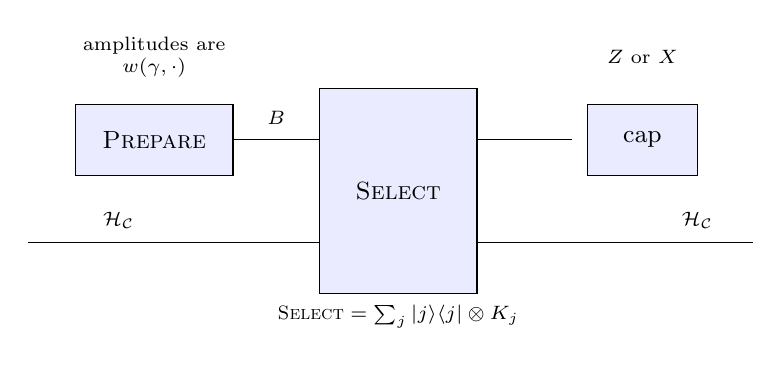
\begin{tikzpicture}[baseline]
  % wires
  \draw[zxw] (-0.6,0) -- (8.6,0);
  \draw[zxw] (1.9,1.3) -- (6.3,1.3);
  % boxes
  \node[zxbox, minimum width=20mm] (prep) at (1.0,1.3) {\PREP};
  \node[zxbox, minimum width=20mm, minimum height=26mm] (sel) at (4.1,0.65) {\SEL};
  \node[zxbox, minimum width=14mm] (cap) at (7.2,1.3) {cap};
  % labels
  \node[font=\scriptsize] at (2.55,1.58) {$B$};
  \node[font=\scriptsize] at (0.55,0.28) {$\Hc$};
  \node[font=\scriptsize] at (7.9,0.28) {$\Hc$};
  \node[font=\scriptsize, align=center] at (1.0,2.35) {amplitudes are\\ $w(\gamma,\cdot)$};
  \node[font=\scriptsize, align=center] at (7.2,2.35) {$Z$ or $X$};
  \node[font=\scriptsize] at (4.1,-0.95) {$\SEL = \sum_j \ketbra{j}{j}\otimes K_j$};
\end{tikzpicture}
\end{center}

The diagram is the whole design in one picture. The term register runs straight through. The
branch register is created by \PREP\ carrying the weight map, is consumed by \SEL\ selecting a
jump, and is then capped. \emph{Which cap} is the semantics, and \S\ref{sec:caps} is about that
choice.

\subsection{Composition to depth \texorpdfstring{$\beta$}{beta}}

\begin{definition}[Budgeted diagram]\label{def:Dbeta}
$D_\beta := (\id_{\Hb^{\otimes\beta}} \otimes \,\cdot\,)$-composite of $\beta$ copies of $V$, with
branch registers $B_1,\dots,B_\beta$ retained:
\[
  D_\beta : \Hc \to \Hb^{\otimes \beta}\otimes\Hc, \qquad
  D_\beta \ket{\gamma_0} = \sum_{j_1,\dots,j_\beta} \Bigl(\prod_{i=1}^{\beta} w(\gamma_{i-1}, j_i)\Bigr)
  \ket{j_1\cdots j_\beta}\otimes\ket{\gamma_\beta},
\]
where $\gamma_i = K_{j_i}\gamma_{i-1}$ and terms with a vanishing $K$ drop out.
\end{definition}

\begin{proposition}[Semigroup]\label{prop:semigroup}
$D_{\beta+1} = (\id_{\Hb^{\otimes\beta}}\otimes V)\circ D_\beta$, and the amplitude attached to
$\ket{j_1\cdots j_\beta}\otimes\ket{\gamma_\beta}$ is the product of the weights along the unique
derivation $j_1,\dots,j_\beta$.
\end{proposition}

\begin{proof}
Immediate from Definition~\ref{def:Dbeta}; uniqueness of the derivation given the branch record
is Proposition~\ref{prop:labels}, since $j_i$ determines $(r,\ell,\kappa)$ and $\ell$ determines
the firing.
\end{proof}

Proposition~\ref{prop:semigroup} is the correctness test we get for free: the compiler is
required to emit diagrams satisfying it, and a differential harness can check
$D_{\beta+1} \overset{?}{=} V \circ D_\beta$ by ZX-rewriting rather than by contraction.

\section{Symbolic execution: the compiler}\label{sec:symbolic}

The diagram of Definition~\ref{def:Dbeta} is configuration-independent, but the jump set and the
address set are not known in advance. Symbolic execution computes them.

\subsection{The frontier}

\begin{definition}[Symbolic state]\label{def:symstate}
A \emph{symbolic state} is a pair $(\Gamma, k)$ where $\Gamma \subseteq \Cfg$ is a set of
configurations, represented as a set of partial tag assignments, and $k \le \beta$ is the number
of steps taken. The initial symbolic state is $(\{\gamma_0\}, 0)$ with
$\gamma_0 = \pi(\sem{t}_\varepsilon)$.
\end{definition}

We do \emph{not} carry amplitudes in the symbolic state. Amplitudes are what the diagram is for;
the executor's job is to discover the address set, the jump set, and the footprints, and to emit
structure. This is the difference between a symbolic executor and a simulator, and it is why the
executor can afford to explore all branches where the simulator of~\cite{weighted} samples one.

\begin{construction}[The compiler]\label{con:compiler}\rm
\begin{enumerate}[leftmargin=2em,label=\arabic*.]
  \item $\Loc \gets$ locations of $\sem{t}_\varepsilon$; $\Gamma \gets \{\gamma_0\}$; $k\gets 0$.
  \item While $k < \beta$:
    \begin{enumerate}[label=2.\arabic*]
      \item For each $\gamma\in\Gamma$, each rule $r$, each $\ell\in\Loc$ with
            $\mathrm{hd}(L_r)$ admissible at $\ell$: determine the refinement class $\kappa$ of
            $\gamma$ under $\mathcal{K}_r$ (unique by Convention~\ref{conv:partition});
            record $j=(r,\ell,\kappa)$, its read set, its write set.
      \item $\Loc \gets \Loc \cup \bigcup_j \mathrm{wr}(j)$.
      \item $\Gamma \gets \{\,K_j\gamma : \gamma\in\Gamma,\ j \text{ enabled at }\gamma\,\}$,
            plus $\gamma$ itself for each $\gamma$ with no enabled jump (the identity jump of
            Convention~\ref{conv:idjump}).
      \item $k \gets k+1$.
    \end{enumerate}
  \item $\Jumps_\beta(t) \gets$ the recorded jumps; $\Loc_\beta(t)\gets\Loc$.
  \item Emit: the qubit layout from $\Loc_\beta(t)$ and $q$; for each step $i\le\beta$ a fresh
        branch register $B_i$; the \PREP\ gadgets of Construction~\ref{con:keygadget}; the
        \SEL\ blocks of Definition~\ref{def:select} using Lemma~\ref{lem:matrixunit}; the cap
        chosen per \S\ref{sec:caps}.
\end{enumerate}
\end{construction}

\begin{proposition}[Termination]\label{prop:terminates}
Construction~\ref{con:compiler} halts after $\beta$ iterations, and $|\Loc_\beta(t)|$ satisfies
the bound of Proposition~\ref{prop:width}.
\end{proposition}

\begin{proof}
The loop is bounded by $\beta$ by construction; each iteration adds at most the write sets of
finitely many jumps, and the growth factor is bounded as in Proposition~\ref{prop:width}.
\end{proof}

\begin{remark}[Cost accounting is the budget]\label{rem:cost}
We have written $\beta$ as a step count for simplicity, but the intended budget is the cost
account of the transpiler branch: the funding judgment $\mathrm{funds}\ \Sigma\ \Delta := \Delta
\le \Sigma$ gates whether a redex is fundable, and an unfundable redex contributes no jump.
Under that reading the identification is exact and pleasing: \emph{the cost budget is the
circuit depth}, and by Proposition~\ref{prop:width} it is also, through the address set, the
circuit width. The classical framework charges cost per rewrite; here the same account
buys wires.
\end{remark}

\subsection{Reflection and drop}\label{ssec:reflection}

The rho calculus of the desugaring uses reflection for two things: freshness, and re-installation
of listeners. Neither escapes the budget.

\emph{Freshness.} Freshness is supplied by quoting, not by $\nu$ and not by a central allocator:
an injected term publishes on a root $@n$ for a quoted nonce $n$, and locations
within it are $@(n,\ell)$~\cite[Rem.~4.4]{knotted}. Fresh addresses are therefore
computable at compile time, and a fresh location is an ancilla register initialised to
$\ket{\mathrm{enc}(\bot)} = \ket{0}^{\otimes q}$. There is no dynamic allocator to model.

\emph{Re-installation.} By Proposition~\ref{prop:listener} the listener family is invariant, so
re-installation contributes no diagram content at all.

\emph{Drop.} A program that dereferences a received name, running received code, is not excluded,
but its address set must be discovered rather than assumed: step 2.2 of
Construction~\ref{con:compiler} adds the locations of whatever is dropped. Within a budget this
is a finite set. The following is the boundary worth stating explicitly.

\begin{proposition}[Reflection is $Z$-copy, and only on the diagonal]\label{prop:nocloning}
Duplication of a quoted term is realised by the $Z$-spider, which copies computational basis
states. It is therefore sound on configurations that are basis states and unsound on
superpositions: there is no linear map duplicating an arbitrary $\ket{\psi}\in\Hc$.
\end{proposition}

\begin{proof}
The $Z$-spider with one input and $n$ outputs sends $\ket{a}\mapsto\ket{a}^{\otimes n}$ for
$a$ in the computational basis, and is linear, so it does not send a superposition to its
tensor power. Non-existence of a general duplicator is the no-cloning theorem.
\end{proof}

The consequence for the compiler is a syntactic side condition rather than a restriction on the
source calculus: a jump whose right-hand side duplicates a hole-filler must be sequenced so that
the duplicated register is in a basis state at the moment of duplication, or the duplication must
be deferred behind a measurement. Programs in which code superposed across branches is duplicated
are outside this compiler.

\section{Three caps and what they mean}\label{sec:caps}

The one-step diagram leaves the branch register open. This section is the note's centre: the
choice of cap is the choice of semantics, and the two principal choices are the two colours of
spider.

\subsection{The \texorpdfstring{$Z$}{Z} cap: the stochastic reading}

\begin{theorem}[$Z$-cap recovers the SSA selection step]\label{thm:classical}
Let $\gamma\in\Cfg$ be a configuration and let $B$ be measured in the computational basis after
$V$. Then outcome $j$ occurs with probability
\[
  \Pr[j] \;=\; \frac{|w(\gamma,j)|^2}{\sum_{j'} |w(\gamma,j')|^2\,\|K_{j'}\ket{\gamma}\|^2}\,
  \|K_j\ket{\gamma}\|^2
  \;=\; \frac{|w(\gamma,j)|^2\,\chi_j(\gamma)}{\sum_{j'} |w(\gamma,j')|^2\,\chi_{j'}(\gamma)},
\]
where $\chi_j(\gamma)\in\{0,1\}$ is enabledness, and the post-measurement state of the term
register is $\ket{K_j\gamma}$. The induced process on $\Cfg$ is the embedded jump chain of the
weighted GSLT with rates $\lambda(w) = |w|^2$.
\end{theorem}

\begin{proof}
$V\ket{\gamma} = \sum_j w(\gamma,j)\ket{j}\otimes K_j\ket{\gamma}$, and the $\ket{j}$ are
orthonormal, so the Born rule gives
$\Pr[j] \propto |w(\gamma,j)|^2\|K_j\ket{\gamma}\|^2$. By
Proposition~\ref{prop:Kcorrect}, $K_j\ket{\gamma}$ is a normalised basis vector when $j$ is
enabled and $0$ otherwise, so $\|K_j\ket{\gamma}\|^2 = \chi_j(\gamma)$. Normalising gives the
stated probability, which is precisely Gillespie's selection of a reaction channel with
probability proportional to its propensity, with propensity $|w|^2$.
\end{proof}

\begin{corollary}[Multiplicity is counted]\label{cor:multiplicity}
If $m$ distinct locations $\ell_1,\dots,\ell_m$ admit the same rule in the same refinement class
with common weight $w$, they contribute $m$ distinct jumps $j_1,\dots,j_m$, and the total
propensity attributed to that channel is $m|w|^2$.
\end{corollary}

\begin{proof}
The jumps are distinct because $c$ is injective (Proposition~\ref{prop:labels}); each contributes
$|w|^2$ to the denominator of Theorem~\ref{thm:classical}.
\end{proof}

Corollary~\ref{cor:multiplicity} is Gillespie's $h$, and it arrives here as a consequence of the
location encoding rather than as a correction that has to be remembered. The central correctness
gap identified in~\cite[\S9.2]{weighted} --- that the prototype omitted multiplicity entirely ---
cannot be reintroduced by a compiler built this way, because there is no representation in which
two redexes at different locations are the same object.

\begin{remark}[Holding times are not in the diagram]\label{rem:holding}
Theorem~\ref{thm:classical} gives the jump chain, not the continuous-time process. The
exponential holding time with parameter $a_0(\gamma) = \sum_j |w(\gamma,j)|^2\chi_j(\gamma)$ is
supplied classically, outside the diagram, exactly as the second random number of the SSA is.
Note that $a_0(\gamma) = \|V\ket{\gamma}\|^2$, so the total propensity is the squared norm of
the one-step image and is readable off the diagram's scalar.
\end{remark}

\subsection{The \texorpdfstring{$X$}{X} cap: the coherent reading}

\begin{theorem}[$X$-cap performs the coherent sum]\label{thm:coherent}
Let $B$ be measured in the $X$ basis after $V$ and the outcome $\ket{+}^{\otimes b}$ retained.
Then, up to the scalar $2^{-b/2}$, the term register carries
\[
  \sum_{j\in\Jumps_\beta(t)} w(\gamma,j)\,K_j\ket{\gamma},
\]
so derivations reaching the same configuration add with the relative phases of their weights,
and the success probability of the post-selection is
$\bigl\|\sum_j w(\gamma,j)K_j\ket{\gamma}\bigr\|^2 / \bigl(2^{b}\bigr)$ relative to the
unnormalised input.
\end{theorem}

\begin{proof}
$\bra{+}^{\otimes b}\ket{j} = 2^{-b/2}$ for every $j$, so
$(\bra{+}^{\otimes b}\otimes\id)V\ket{\gamma} = 2^{-b/2}\sum_j w(\gamma,j)K_j\ket{\gamma}$. The
success probability is the squared norm of the retained branch over the squared norm of the
whole.
\end{proof}

\begin{corollary}[Interference is exactly diamond closure]\label{cor:diamond}
Two jumps $j\neq j'$ enabled at $\gamma$ contribute to the same amplitude under
Theorem~\ref{thm:coherent} if and only if $K_j\ket{\gamma} = K_{j'}\ket{\gamma}$, i.e.\ iff the
local diamond at $\gamma$ closes in one step.
\end{corollary}

\begin{proof}
The sum $\sum_j w(\gamma,j)K_j\ket{\gamma}$ groups terms by the basis vector
$K_j\ket{\gamma}$; two terms share a coefficient exactly when they share that vector.
\end{proof}

Corollary~\ref{cor:diamond} recovers, in the compiled setting, the proposition of~\cite{weighted}
identifying interference with closed local diamonds --- but with the roles of confluence and
non-confluence now clear. A confluent calculus is one all of whose diamonds close, hence one in
which the $X$-cap has a great deal to do; the lambda calculus presented with contextual rules at
every position is the interference-rich case, not the degenerate one. A deterministic calculus,
such as a Turing machine, has a single derivation, so the sum has one term, no diamond closes
because none opens, and the compiled diagram is a reversible computation with phases along a
line. A non-confluent calculus --- $\pi$, rho, the ambient calculus --- has diamonds that do not
close; those branches reach distinct configurations and therefore do not interfere, and what to
do with them is the third cap.

\subsection{The term register: operational non-determinism}

Genuine non-confluence produces a superposition over distinct configurations. If the intended
semantics of the source is that the program makes a non-deterministic choice --- which is what
the operational semantics of a mobile process calculus says --- then that superposition must be
resolved, and resolving it is a measurement of the term register. This is the sense in which
measurement matches the program semantics rather than repairing the encoding.

\begin{table}[t]
\centering
\small
\begin{tabular}{@{}lll@{}}
\toprule
\textbf{Cap} & \textbf{Denotes} & \textbf{Semantics recovered} \\
\midrule
$B$ measured in $Z$ & $\sigma \mapsto \sum_j |w_j|^2 K_j\sigma K_j^\dagger$ & Gillespie / SSA jump chain \\
$B$ post-selected in $X$ & $\ket{\psi}\mapsto \sum_j w_j K_j\ket{\psi}$ & coherent sum over derivations \\
$B$ retained & isometry $V$ (if uniformised) & unitary dilation, no interference \\
term register measured & collapse to a configuration & operational non-determinism \\
\bottomrule
\end{tabular}
\caption{The four terminations of one diagram.}\label{tab:caps}
\end{table}

\begin{remark}[Multiplicity, revisited]\label{rem:mult}
Let $m$ derivations reach a common target as in Corollary~\ref{cor:multiplicity}. Under the $Z$
cap the target is reached with total probability $\propto m|w|^2$: the classical answer, linear
in $m$. Under the $X$ cap the amplitude is $mw$ and the weight $m^2|w|^2$: superlinear.
The earlier note identified $m^2$ as a normalisation artefact and repaired it by taking one
square root of the summed rate rather than summing square roots. That repair was correct
\emph{for the construction it repaired}, in which the $m$ derivations had no separate
representation and the degeneracy was double-counted. Here the situation is different: the $m$
derivations are $m$ distinct basis vectors of $B$, distinguished by injectivity of $c$, and the
two answers are not competing normalisations of one quantity but the values of two different
observables. Linear in $m$ is what you get when you look at which derivation fired; quadratic in
$m$ is what you get when you decline to look. The $m^2$ is the signature of coherent
recombination, and it is correct exactly when the recombination is real.
\end{remark}

\section{Which-path, and why measurement is the engine}\label{sec:whichpath}

The reader may reasonably ask why the branch register must be capped at all --- why not
uncompute it, coherently, and keep everything unitary. The answer is that it cannot be done, and
the reason is worth stating as a theorem because it determines the architecture.

\begin{theorem}[Which-path]\label{thm:whichpath}
Suppose $j \neq j'$ are enabled at $\gamma$ with $K_j\ket{\gamma} = K_{j'}\ket{\gamma}$. Then:
\begin{enumerate}[leftmargin=*,label=(\roman*)]
  \item With $B$ retained, the reduced state of the term register is
        $\sum_j |w_j|^2 K_j\ketbra{\gamma}{\gamma}K_j^\dagger$, in which the $j$ and $j'$ terms
        add incoherently: no interference occurs.
  \item There is no unitary $U$ on $\Hb$ with $U\ket{j} = U\ket{j'} = \ket{0}$.
  \item Hence the only maps that recombine $j$ and $j'$ coherently are non-unitary: projections
        (equivalently, post-selected measurements).
\end{enumerate}
\end{theorem}

\begin{proof}
(i) Tracing out $B$ from $V\ketbra{\gamma}{\gamma}V^\dagger$ kills the off-diagonal terms
$\ketbra{j}{j'}$ because the $\ket{j}$ are orthonormal, leaving the stated Kraus form.
(ii) A unitary is injective; $\ket{j}\neq\ket{j'}$ cannot have the same image.
(iii) By (i) coherence requires the off-diagonal terms to survive, which requires $B$ not to be
traced out; by (ii) they cannot be brought to a common basis vector unitarily; a linear map
sending $\ket{j}$ and $\ket{j'}$ to a common vector is non-injective, hence non-unitary, and the
$X$-basis effect $\bra{+}$ of Theorem~\ref{thm:coherent} is such a map.
\end{proof}

Theorem~\ref{thm:whichpath} deserves emphasis because it inverts the usual expectation. In this
architecture measurement is not a concession made because programs fail to be unitary. It is the
only operation that can merge derivations, and merging derivations is what interference
\emph{is}. The remark that not all programs deliver unitary matrices, and that we should be able
to avail ourselves of measurement, is therefore not a caveat attached to the design; it is the
design.

\begin{corollary}[No third semantics]\label{cor:nothird}
Any cap on $B$ is a linear map $\Hb\to\mathbb{C}$ (or a measurement thereof). The $Z$-basis
measurements give Theorem~\ref{thm:classical}, the $\bra{+}$ effect gives
Theorem~\ref{thm:coherent}, and intermediate bases interpolate: capping with
$\bra{\theta} = \sum_j e^{-i\theta_j}\bra{j}/\sqrt{N}$ gives
$\sum_j e^{-i\theta_j}w_jK_j\ket{\gamma}/\sqrt{N}$, i.e.\ a coherent sum with the weight map
rotated by $\theta$.
\end{corollary}

Corollary~\ref{cor:nothird} says the cap is not a binary switch but a dial, and that the dial is
in the same space as the weight map. A partial cap --- measuring some qubits of $B$ and
post-selecting others --- decoheres a chosen quotient of the derivations, which is exactly the
apparatus needed to say ``these derivations interfere, those merely branch''. We do not develop
the partial case here; it is the natural home for a treatment of decoherence induced by
observation of a shard.

\section{Unitarity, dilation, extraction}\label{sec:unitary}

Everything so far denotes a linear map, which is all a ZX diagram ever needs to do, and is
enough for the simulation and rewriting half of the programme. Running on hardware needs more.
This section says exactly how much more.

\subsection{Uniformisation}

\begin{definition}[Uniformised weight map]\label{def:uniform}
$w$ is \emph{uniformised} on a set $S\subseteq\Cfg$ if for every $\gamma\in S$,
$\sum_{j} |w(\gamma,j)|^2\chi_j(\gamma) = 1$.
\end{definition}

\begin{theorem}[Dilation]\label{thm:dilation}
If $w$ is uniformised on the configurations reachable within the budget, then
$V:\Hc\to\Hb\otimes\Hc$ of Definition~\ref{def:V} is an isometry, and hence extends to a unitary
$\tilde{V}$ on $\Hb\otimes\Hc$.
\end{theorem}

\begin{proof}
$V^\dagger V = \sum_{j,j'}\overline{w_j}w_{j'}\bra{j}j'\rangle K_j^\dagger K_{j'}
= \sum_j |w_j|^2 K_j^\dagger K_j$. By Definition~\ref{def:K},
$K_j^\dagger K_j = \ketbra{\hat{L}_\ell}{\hat{L}_\ell}\otimes\id$, the projector onto
configurations at which $j$ is enabled, so
$V^\dagger V\ket{\gamma} = \bigl(\sum_j|w(\gamma,j)|^2\chi_j(\gamma)\bigr)\ket{\gamma}
= \ket{\gamma}$ by hypothesis. An isometry into a space of dimension
$\dim\Hb\cdot\dim\Hc > \dim\Hc$ extends to a unitary by completing the image's orthonormal basis.
\end{proof}

\begin{proposition}[Totality needs the identity jump]\label{prop:idneeded}
Without Convention~\ref{conv:idjump}, no weight map is uniformised on a set containing a normal
form.
\end{proposition}

\begin{proof}
At a normal form no jump is enabled, so the sum in Definition~\ref{def:uniform} is empty and
equals $0\neq 1$.
\end{proof}

The fictitious-jump convention of~\cite{weighted} therefore acquires a second, sharper
justification: it was introduced so that the generator's diagonal and the SSA's total propensity
would agree on self-transitions, and it turns out to be exactly what makes the quantum step
total. A normal form must be a fixed point with weight of modulus one, or the machine has nothing
to do and no unitary describes it.

\begin{remark}[{$[0,1]$ versus $\mathbb{R}_{\geq 0}$, resolved}]\label{rem:clamp}
The earlier note debated whether the weight codomain should be the unit interval or
$\mathbb{R}_{\geq 0}$, settled on the latter, and removed the $|z|\le 1$ clamp. Both decisions
stand. Uniformisation is a different and weaker condition: it does not bound individual weights,
it constrains their sum per configuration. It is the quantum counterpart of \emph{uniformisation}
in the Markov-chain sense --- converting a CTMC to a DTMC with a uniform clock --- and the
present theorem says that uniformisation is precisely the price of extractability. Weight maps
that are not uniformised are perfectly good diagrams; they are simply not circuits.
\end{remark}

\subsection{Predicate-and-permutation form}\label{ssec:predperm}

Theorem~\ref{thm:dilation} guarantees a unitary extension abstractly. To hand PyZX something it
can extract, the extension must be realised. The following decomposition does it, at the price of
a syntactic condition on the rule set.

\begin{construction}[Predicate and permutation]\label{con:predperm}\rm
Write $K_j = U_j P_j$ where $P_j = \ketbra{\hat{L}_\ell}{\hat{L}_\ell}\otimes\id$ is the
enabledness projector and $U_j$ is any permutation of $\Tagsb^{\fp(j)}$ sending $\hat{L}_\ell$ to
$\hat{R}_\ell$, extended by the identity. Then:
\begin{enumerate}[leftmargin=2em,label=\arabic*.]
  \item $\MATCH_j$: a reversible circuit computing $\chi_j$ into a flag $f_j$, from
        $\pi_{\mathrm{rd}(j)}$. Comparison against a constant bit string; Toffoli depth
        $O(q\,|\mathrm{rd}(j)|)$.
  \item $\WRITE_j$: $U_j$ controlled on $f_j$ and on $B=j$. A controlled permutation, hence a
        reversible circuit.
  \item $\MATCH_j^{-1}$: uncompute $f_j$ by testing whether the footprint now matches
        $\hat{R}_\ell$.
\end{enumerate}
\end{construction}

\begin{definition}[Write-detectability]\label{def:writedetect}
A rule set is \emph{write-detectable} if for every $j$, and every configuration $\gamma$, the
footprint of $j$ matches $\hat{R}_\ell$ after $\WRITE_j$ if and only if it matched
$\hat{L}_\ell$ before. Equivalently, no configuration matches both $\hat{L}_\ell$ and
$\hat{R}_\ell$ at $\ell$.
\end{definition}

\begin{proposition}[Flag uncomputation]\label{prop:flag}
If the rule set is write-detectable, step 3 of Construction~\ref{con:predperm} returns $f_j$ to
$\ket{0}$, and the composite $\MATCH_j^{-1}\WRITE_j\MATCH_j$ is a unitary on
$\Hb\otimes\Hc$ agreeing with $\ketbra{j}{j}\otimes K_j$ on the enabled subspace.
\end{proposition}

\begin{proof}
Write-detectability makes the post-write test the same Boolean function of the post-write state
as the pre-write test was of the pre-write state, so the second $\MATCH$ XORs the same bit into
$f_j$ and clears it. Each of the three factors is reversible, so the composite is.
\end{proof}

If a rule set is not write-detectable --- a rule whose right-hand side can look like its own
left-hand side, of which the identity jump is the extreme case --- the flag cannot be uncomputed
and is garbage. Garbage is discarded, which decoheres, which returns us to
Theorem~\ref{thm:whichpath}: the failure of write-detectability is precisely a failure to be able
to tell which derivation ran, and the diagram registers it as such. The identity jump is exempt
because it is a fixed point and needs no flag.

\subsection{What is actually extractable}

Stacking the conditions gives a three-tier statement, which we record as the honest answer to
``when can this run on hardware''.

\begin{enumerate}[leftmargin=*]
  \item \emph{Always.} A $\cwG$ program plus a budget compiles to a ZX diagram denoting a linear
        map. No conditions. This is the tier at which PyZX rewriting and classical simulation by
        contraction apply.
  \item \emph{Under uniformisation.} $V$ is an isometry and dilates
        (Theorem~\ref{thm:dilation}); under write-detectability the dilation is realised by
        Construction~\ref{con:predperm} as a reversible circuit plus phase gadgets.
  \item \emph{Under extraction.} The simplified diagram must additionally admit a gflow (or
        another correctability condition) for PyZX's circuit extraction to succeed. Simplification
        does not preserve circuit-likeness, so this is checked after simplification, not before.
        Where it fails, the diagram remains a measurement pattern with post-selection, and
        post-selection costs sampling overhead exponential in the number of post-selected
        qubits.
\end{enumerate}

Tier 3 is why hardware is a later back end rather than a near-term target, and the note does not
claim otherwise. The immediate value is tiers 1 and 2: a compiled, simplifiable, contractible
object with a proof obligation attached to each of its two possible caps.

\section{A worked example: a coherent spiking network}\label{sec:network}

The weighted-GSLT note carried a spiking network as its worked example, with
synaptic weights living in the weight map rather than in the payload and
plasticity as the map's update function. We keep that skeleton and change the
codomain to $\mathbb{C}$. The question this section answers is what the phase
buys, and the answer is that it correlates neurons.

Everything below is contracted out of an emitted ZX diagram. Section
\ref{ssec:machinery} says how; \S\ref{ssec:numbers} gives the numbers, which are
cross-checked against an independently written implementation of
Definition~\ref{def:Dbeta} to a worst deviation of $8.9\times 10^{-16}$.

\subsection{The theory}\label{ssec:theory}

Take a one-constructor signature, so $|\Tags| + 1 = 2$ and $q = 1$: a location
either carries a spike or does not. Locations are two release sites $s_1, s_2$
and two somas $a, b$. For $x \in \{1,2\}$ and $y \in \{a,b\}$ there are two
rules,
\[
  \mathrm{relay}(x,y) \;:\; s_x{=}1,\, y{=}0 \;\rew\; s_x{=}0,\, y{=}1,
  \qquad
  \mathrm{leak}(x,y) \;:\; s_x{=}1,\, y{=}1 \;\rew\; s_x{=}0,\, y{=}1 .
\]
Transmission moves a spike from a release site to a silent soma; a spike
arriving at a soma that is already spiking is lost. The leak rule is not
decoration: without it the only reachable configuration after two firings is
$(a{=}1, b{=}1)$ and there is nothing to correlate. It is also the repair the
earlier note arrived at independently, where a hard capacity made a saturating
network absorbing rather than live.

The jump index is $j = (r,x,y)$ with $r \in \{\mathrm{relay},\mathrm{leak}\}$,
so $|\Jumps| = 8$ and the branch register is three qubits per step. The weight
map is
\[
  w(\mathrm{relay}, x, y) = t_{xy}, \qquad w(\mathrm{leak}, x, y) = \lambda ,
\]
with $t$ a $2\times 2$ matrix of synaptic amplitudes. The budget is $\beta = 2$:
exactly enough to consume both spikes.

\begin{proposition}[The co-firing configuration is a closed diamond]\label{prop:cofire}
The configuration $(a{=}1, b{=}1)$ is reached from $(s_1{=}1, s_2{=}1, a{=}0,
b{=}0)$ by exactly four derivations of length two --- two pairings of spikes to
somas, each in two orders --- with amplitudes
$t_{1a}t_{2b}$, $t_{1b}t_{2a}$, $t_{2b}t_{1a}$, $t_{2a}t_{1b}$.
The configurations $(1,0)$ and $(0,1)$ are reached by two derivations each,
with amplitudes $\lambda t_{1y}$ and $\lambda t_{2y}$. The configuration
$(0,0)$ is unreachable, since $\mathrm{leak}$ is disabled at a silent soma.
\end{proposition}

\begin{proof}
Direct enumeration of the two-step derivations, using
Proposition~\ref{prop:Kcorrect} for enabledness.
\end{proof}

By Corollary~\ref{cor:diamond} the four co-firing amplitudes interfere under the
$X$ cap and do not under the $Z$ cap. That is the whole example.

\subsection{What is emitted, and how it is contracted}\label{ssec:machinery}

The emitter follows \S\ref{sec:zx} without shortcuts. \PREP\ is realised by the
multiplexed-rotation state preparation of a general $n$-qubit amplitude vector,
so the weight map really is a state on the branch register and not a
post-processing step. \SEL\ is realised in the predicate-and-permutation form of
Construction~\ref{con:predperm}: a reversible $\MATCH$ writes
$\chi_{j(B)}(\gamma)$ into a flag from the read set, the flag is left in place,
$\WRITE$ applies the controlled permutation, and the flag is capped with a
$\ket{1}$ effect. That effect is the projection: branch records whose selected
jump is disabled are annihilated rather than acting as the identity, which is
the distinction Construction~\ref{con:predperm} otherwise leaves open. Of the
$64$ two-step branch records, $8$ survive it.

The emitted diagram for the two-step network has $1806$ vertices and $2244$
edges. Two engineering findings are worth recording because they bear on
\S\ref{sec:impl}'s recommendation.

\begin{remark}[Contraction order, not diagram size, is the bottleneck]\label{rem:contract}
A contraction that walks the vertices in order is unusable here: on the reduced
$118$-vertex diagram it demands a $64$\,GiB intermediate. Emitting each spider
at bond dimension two --- a spider of degree $d$ is $\sum_k c_k \ket{k}^{\otimes
d}$, hence a chain of rank-three copy tensors rather than a dense rank-$d$
array --- and choosing the path by a standard optimiser contracts the same
diagram in seconds. Any implementation of \S\ref{sec:impl} should provide its
own contractor and not rely on the reference one.
\end{remark}

\begin{remark}[Simplification can make contraction harder]\label{rem:reduce}
Full simplification takes the network diagram from $1806$ vertices to $118$, and
makes it \emph{harder} to contract: the reduced diagram exceeds memory where the
unreduced one contracts in about three seconds. Simplification trades vertex
count for connectivity, and contraction cost is governed by treewidth. This cuts
against the natural assumption that simplification is always the first move; on
the minimal diagram of \S\ref{ssec:numbers} it is an unambiguous win ($10$
vertices to $2$, tensor preserved), and on the network diagram it is not.
\end{remark}

\subsection{The numbers}\label{ssec:numbers}

\paragraph{Convergent input, and inhibition as a phase.}
First the minimal closed diamond: one release site, two rules with identical
left- and right-hand sides --- two synaptic routes to one soma --- so
$K_{j_1} = K_{j_2}$ and the diamond closes in a single step. Contracting the
one-step diagram of Definition~\ref{def:V} under each cap:

\begin{center}
\small
\begin{tabular}{@{}lccc@{}}
\toprule
& relative phase & $Z$ cap: $\sum_j |w_j|^2$ & $X$ cap: $|\sum_j w_j|^2$ \\
\midrule
excitatory   & $0$       & $1.000000$ & $2.000000$ \\
inhibitory   & $\pi$     & $1.000000$ & $0.000000$ \\
quadrature   & $\pi/2$   & $1.000000$ & $1.000000$ \\
one route    & ---       & $1.000000$ & $1.000000$ \\
\bottomrule
\end{tabular}
\end{center}

\begin{remark}[Inhibition needs no negative rate]\label{rem:inhibition}
The classical framework has weights in $\mathbb{R}_{\geq 0}$, so inhibition must
be encoded structurally --- a capacity guard, a competing consumer, a leak.
Here it is a relative phase of $\pi$ on a synapse and it cancels exactly, by the
same mechanism that produces excitation. This is the smallest thing the complex
codomain buys that the real one cannot express at all.
\end{remark}

\paragraph{Two spikes, two neurons.}
Now the network of \S\ref{ssec:theory}, with $\lambda = 1/\sqrt{2}$ and two
weight maps of \emph{identical magnitudes}: a beamsplitter
$t = \frac{1}{\sqrt2}\left(\begin{smallmatrix} 1 & 1 \\ i & -i
\end{smallmatrix}\right)$ and its phase-free counterpart
$t = \frac{1}{\sqrt2}\left(\begin{smallmatrix} 1 & 1 \\ 1 & 1
\end{smallmatrix}\right)$.

\begin{center}
\small
\begin{tabular}{@{}lccc@{}}
\toprule
outcome $(a,b)$ & $Z$ cap (both maps) & $X$ cap, beamsplitter & $X$ cap, phase-free \\
\midrule
$(1,1)$ both fire   & $0.500000$ & $\mathbf{0.000000}$ & $0.666667$ \\
$(1,0)$ only $a$    & $0.250000$ & $0.500000$ & $0.166667$ \\
$(0,1)$ only $b$    & $0.250000$ & $0.500000$ & $0.166667$ \\
\midrule
$\mathrm{corr}(a,b)$ & $-1/3$ & $-1$ & $-1/5$ \\
\bottomrule
\end{tabular}
\end{center}

The left column is the point. The two weight maps are indistinguishable under
the $Z$ cap, because $\lambda(z) = |z|^2$ is the same for both; they induce the
same jump chain, the same propensities, the same Gillespie simulation. Under the
$X$ cap the beamsplitter phases drive co-firing to exactly zero --- the two
neurons never both fire, and the two spikes always land on the same soma ---
while phase-free weights of the same magnitude \emph{enhance} co-firing to
$2/3$. The correlation runs from $-1$ through $-1/3$ to $-1/5$.

\begin{proposition}[The coherent law is unreachable classically]\label{prop:unreachable}
No weight map with values in $\mathbb{R}_{\geq 0}$ on the theory of
\S\ref{ssec:theory} produces $\Pr[(1,1)] = 0$ while leaving
$\Pr[(1,0)], \Pr[(0,1)] > 0$, under either cap.
\end{proposition}

\begin{proof}
Under the $Z$ cap the four co-firing derivations of
Proposition~\ref{prop:cofire} contribute $\sum |t_{1y}t_{2y'}|^2 > 0$ whenever
any $t$ is nonzero, and $\Pr[(1,0)]>0$ forces some $t_{\cdot a} \neq 0$. Under
the $X$ cap the co-firing amplitude is $2(t_{1a}t_{2b} + t_{1b}t_{2a})$, a sum
of products of non-negative reals, which vanishes only if $t_{1a}t_{2b} =
t_{1b}t_{2a} = 0$; that in turn forces one of $\Pr[(1,0)], \Pr[(0,1)]$ to
vanish.
\end{proof}

Proposition~\ref{prop:unreachable} is the honest form of the claim. It is not
that this network violates a bound on all classical models --- a classical model
with correlated routing reproduces the marginals easily --- but that within the
weighted-GSLT framework, on a fixed theory, the transition from enhanced
co-firing to zero co-firing is reachable by the phase and by nothing else.

\begin{remark}[Bunching, and the $m^2$ thread]\label{rem:bunching}
The coherent outcome is that the two spikes always co-locate. This is the
bosonic enhancement that the earlier note raised and closed as a normalisation
artefact, reappearing where it is not an artefact:
Remark~\ref{rem:mult}'s $m^2$ is bunching, and here the derivations it enhances
are genuinely distinct --- distinguished by injectivity of $c(\ell)$ --- and
genuinely rejoining. The classical linear-in-$m$ answer and the coherent
quadratic-in-$m$ answer are the $Z$ and $X$ columns of the same table.
\end{remark}

\subsection{Plasticity reads the branch record}\label{ssec:plasticity}

In the earlier note plasticity was the weight map's update function, and its
distinguishing feature was that the map may change as the system runs. Under
Definition~\ref{def:prepare} that is a different \PREP\ state at each step,
which \S\ref{ssec:keys} already handles. What is new here is what the update
must \emph{read}.

A Hebbian rule updates $w(\mathrm{relay},x,y)$, so it must know which synapse
carried the spike --- both the presynaptic index $x$ and the postsynaptic index
$y$. By Proposition~\ref{prop:labels} that information lives in the branch
record, and by Theorem~\ref{thm:whichpath} reading it is reading a which-path
record. We model a partial read: a trace register coupled to the step-one
branch bits by a rotation of angle $\alpha$, so that the two trace states have
overlap $c = \cos\alpha$, and then discarded.

The first thing to establish is that the read has to be specific to do damage.

\begin{lemma}[Single-index reads are free]\label{lem:coarse}
For the beamsplitter of \S\ref{ssec:numbers}, the four co-firing amplitudes are
$-\tfrac{i}{2}, +\tfrac{i}{2}, +\tfrac{i}{2}, -\tfrac{i}{2}$ under the labelling
of Proposition~\ref{prop:cofire}. Grouping them by the presynaptic index alone,
or by the postsynaptic index alone, partitions them into two blocks each
containing one amplitude of each sign. Hence each block sums to zero, and
decohering either index alone leaves $\Pr[(1,1)] = 0$ unchanged.
\end{lemma}

\begin{proof}
Direct computation of the four products, then inspection of the two
one-bit partitions.
\end{proof}

So a plasticity rule that records only which neuron fired, or only which release
site emptied, costs nothing. A rule that records the synapse --- both indices,
which is what a synapse-specific update requires --- separates all four
derivations. Contracting the diagram with both step-one branch bits coupled to
the trace register at strength $\alpha$:

\begin{center}
\small
\begin{tabular}{@{}rrrr@{}}
\toprule
$\alpha$ & $c = \cos\alpha$ & $\Pr[\text{both fire}]$ & $\mathrm{corr}(a,b)$ \\
\midrule
$0$        & $1.000000$ & $0.000000$ & $-1.000000$ \\
$\pi/16$   & $0.980785$ & $0.000369$ & $-0.999262$ \\
$2\pi/16$  & $0.923880$ & $0.005761$ & $-0.988544$ \\
$3\pi/16$  & $0.831470$ & $0.027618$ & $-0.946248$ \\
$4\pi/16$  & $0.707107$ & $0.079009$ & $-0.853553$ \\
$5\pi/16$  & $0.555570$ & $0.164939$ & $-0.716828$ \\
$6\pi/16$  & $0.382683$ & $0.275929$ & $-0.567486$ \\
$7\pi/16$  & $0.195090$ & $0.393160$ & $-0.435586$ \\
$8\pi/16$  & $0.000000$ & $0.500000$ & $-0.333333$ \\
\bottomrule
\end{tabular}
\end{center}

At $c = 0$ the network sits exactly on the $Z$-cap row of
\S\ref{ssec:numbers}: $0.500000$ and $-1/3$. The curve has a closed form.

\begin{proposition}[The exchange rate]\label{prop:exchange}
Let $\eta = 1 - c$ measure the distinguishability the plasticity read achieves.
Then, for the theory and weight map above,
\[
  \Pr[\text{both fire}] \;=\; \frac{\eta^{2}}{1 + \eta^{2}} .
\]
\end{proposition}

\begin{proof}
By Proposition~\ref{prop:cofire} the co-firing weight is
$\sum_{d,d'} A_d \overline{A_{d'}} \langle T_{d'} | T_d\rangle$ over the four
derivations, with $A \in \{-\tfrac{i}{2}, \tfrac{i}{2}, \tfrac{i}{2},
-\tfrac{i}{2}\}$ and trace overlaps $c^{k}$ where $k$ is the number of indices
in which the two derivations differ. The four diagonal terms give $1$; the four
pairs differing in one index give $-c/2$ each; the two pairs differing in both
give $+c^2/2$ each. The total is $1 - 2c + c^2 = (1-c)^2$. The single-soma
outcomes are unaffected --- their two derivations differ in the presynaptic
index only, and their cross term has vanishing real part --- contributing
$1/2$ each. Normalising gives the claim.
\end{proof}

The closed form is verified against the contracted diagram at every row of the
table to a worst deviation of $1.67\times 10^{-16}$.

\begin{corollary}[Learning decoheres]\label{cor:learn}
A synapse-specific plasticity rule on this network destroys the coherent
correlation at the rate $\eta^2/(1+\eta^2)$, reaching the classical law exactly
at $\eta = 1$. The correlation coefficient runs monotonically from $-1$ to
$-1/3$.
\end{corollary}

This is Theorem~\ref{thm:whichpath} in a network. The branch register is what
makes derivations distinguishable, distinguishability is what plasticity needs,
and distinguishability is what interference cannot survive. Lemma~\ref{lem:coarse}
keeps the statement from being vacuous: it is not that observation in general
decoheres, but that observation at exactly the granularity a Hebbian update
requires does, while coarser observation is free. Whether a useful learning rule
exists in the gap --- specific enough to update a synapse, coarse enough to
leave the interfering derivations unresolved --- is the question this example
raises and does not answer.

\begin{remark}[Where the nonlinearity comes from]\label{rem:nonlinear}
A standing objection to any quantum network model is that linear maps cannot
threshold. Nothing in this section adds a nonlinearity by hand, and none is
needed: the McCulloch--Pitts threshold is the join pattern, the join pattern is
the demanded tag assignment $\hat{L}_\ell$ of Definition~\ref{def:K}, and that
is a projector --- linear on $\Hc$, and a Boolean conjunction on configurations.
The Born rule supplies a second, quadratic nonlinearity at the cap. The
framework has two sources of nonlinearity before anyone asks for one.
\end{remark}

\section{Costs and tractable fragments}\label{sec:costs}

\subsection{Width, depth, ancillas}

\begin{proposition}[Resource count]\label{prop:resources}
The diagram $D_\beta$ uses
\[
  \underbrace{q\,|\Loc_\beta(t)|}_{\text{term register}} \;+\;
  \underbrace{\beta\lceil\log_2 N\rceil}_{\text{branch registers}} \;+\;
  \underbrace{\beta\,\max_j |\mathrm{rd}(j)|}_{\text{match flags}}
\]
qubits, where $N = |\Jumps_\beta(t)|$, and has depth $O(\beta\cdot\max_j q|\fp(j)|)$ up to the
Toffoli decomposition of the match predicates.
\end{proposition}

\begin{proof}
Immediate from Construction~\ref{con:compiler} and Construction~\ref{con:predperm}; flags are
reusable across steps when write-detectability holds, giving the stated $\beta$-linear rather
than $\beta$-quadratic count.
\end{proof}

The branch registers are the price of keeping derivations distinct, and by
Theorem~\ref{thm:whichpath} it is not a price that can be avoided by cleverness: the record has
to exist in order to be capped. What can be reduced is $N$. Two observations follow.

\subsection{The Clifford fragment}

\begin{proposition}[Clifford weight maps]\label{prop:clifford}
Suppose $|w(\gamma,j)|$ is independent of $j$ and $\arg w(\gamma,j)\in\frac{\pi}{2}\mathbb{Z}$
for all $\gamma,j$. Then every \PREP\ stage is a Clifford operation on $B$, and the only
non-Clifford content of $D_\beta$ is in the match predicates and the matrix units.
\end{proposition}

\begin{proof}
Under uniform magnitudes $\ket{\mathrm{prep}(\gamma)} \propto D(\gamma)\ket{+}^{\otimes b}$ with
$D$ diagonal with entries in $\{1,i,-1,-i\}$, which is Clifford; $\ket{+}^{\otimes b}$ is
Clifford state preparation.
\end{proof}

This gives a design constraint with teeth. Stabiliser decomposition makes contraction of a ZX
diagram efficient in the number of non-Clifford phases, so a $\cwG$ whose weight phases are
multiples of $\pi/2$ is classically simulable at a cost governed by the remaining $T$-count,
while a weight map with generic phases is not. It is a genuine fragment of the calculus, defined
by a condition on the weight map rather than on the syntax, and it is where a first
implementation should live. The analogy to the ideal-versus-checkable methodology
of~\cite{weighted} is exact: the ideal weight codomain is $\mathbb{C}$, and $\frac{\pi}{2}
\mathbb{Z}$-phases with uniform magnitude is a fragment that computes.

\subsection{Sparsity}\label{ssec:sparsity}

Proposition~\ref{prop:width} is the practical limit, and its cause is that the encoding is dense:
every location in the address set gets $q$ qubits for the whole run, including locations that are
$\bot$ at every reachable configuration except a few. Three mitigations, in increasing order of
ambition and decreasing order of confidence:

\begin{enumerate}[leftmargin=*]
  \item \emph{Location pruning.} Construction~\ref{con:compiler} already computes the reachable
        set; locations that are $\bot$ throughout can be deleted rather than allocated.
  \item \emph{Register reuse.} A location that becomes $\bot$ and is never revisited can have its
        register recycled, provided it is returned to $\ket{0}^{\otimes q}$, which is an
        uncomputation and is subject to the same detectability question as
        Proposition~\ref{prop:flag}.
  \item \emph{Second quantisation.} Where a calculus is presented so that the interesting
        quantity is an occupancy count at a name rather than a tag at a location --- the reading
        under which the earlier note's birth--death and spiking-network examples are natural ---
        one may replace $\mathbb{C}^{\Tagsb}$ per location by a truncated number state per name,
        with the truncation bounded by the copy-number and namespace-scope analysis. We flag this
        as the correct direction for the chemical-reaction-network style of example and do not
        develop it here.
\end{enumerate}

\section{Implementation}\label{sec:impl}

\subsection{Emission}

The compiler's output is a ZX diagram, and there are two reasonable serialisations.

\begin{enumerate}[leftmargin=*]
  \item \emph{Direct PyZX graph.} Emit vertices with type ($Z$, $X$, boundary, Hadamard), phase
        as a fraction of $\pi$, and edges with type (simple, Hadamard), plus a global scalar.
        This is the shortest path to \texttt{full\_reduce}, \texttt{extract\_circuit}, and the
        tensor-based equality check for small instances. The PyZX API and its graph JSON should be
        pinned by version; we do not rely here on any specific serialisation detail.
  \item \emph{A monoidal intermediate.} Emit into a general symmetric-monoidal term
        representation with ZX as one interpretation, and generate PyZX from that. This costs a
        layer and buys the option of retargeting to a calculus with a primitive for linear
        combination, which would let \S\ref{ssec:onestep} drop the branch register in favour of a
        native sum. Given Theorem~\ref{thm:whichpath} that trade is less attractive than it first
        appears --- the branch register is not merely an encoding device, it is where the
        semantics is chosen --- but the option has independent value for the qudit question of
        Remark~\ref{rem:qudits}.
\end{enumerate}

We recommend (1) for the first implementation and (2) only if the qudit or linear-combination
questions become pressing.

\subsection{The pipeline}

\begin{enumerate}[leftmargin=*]
  \item $\cwG$ program $+$ budget $\longrightarrow$ Construction~\ref{con:compiler}
        $\longrightarrow$ address set, jump set, footprints.
  \item $\longrightarrow$ ZX diagram $D_\beta$ with the branch wires open.
  \item Choose a cap (Table~\ref{tab:caps}).
  \item Simplify. Verify against the reference by contraction for small instances.
  \item Attempt extraction; on success, a circuit; on failure, a measurement pattern.
\end{enumerate}

\subsection{What changes in the existing crate}

The weighted simulator \texttt{rho-weighted} is a simulator, not an interpreter, and it owns its
own state; the compiler described here is a third artefact with the same relationship to both. It
shares the parts of the simulator that are about the calculus and shares none of the parts that
are about sampling. Concretely:

\begin{itemize}[leftmargin=*]
  \item \emph{Reused as-is.} The \texttt{Formula} AST and its structural fragment; the R3
        machinery (\texttt{is\_structural}, \texttt{Checkable::try\_key},
        \texttt{Partition::from\_checked\_keys}) --- which \S\ref{ssec:keys} shows to be a
        prerequisite rather than a hygiene measure; the partition check; the exhaustive graph
        construction, which becomes the reference oracle for the differential tests below.
  \item \emph{Generalised.} \texttt{RateValue::complex} loses its interpretation as an amplitude
        of a jump operator and becomes an amplitude of a \PREP\ state; \texttt{rate()} returning
        $|z|^2$ remains correct but is now specifically the $Z$-cap reading
        (Remark~\ref{rem:codomain}).
  \item \emph{New.} The address-set computation of Construction~\ref{con:compiler}; the footprint
        calculation of Definition~\ref{def:footprint}; the qubit layout; the ZX emitter.
  \item \emph{Not reused.} \texttt{QctmcModel} and the Lindblad/quantum-jump apparatus. The
        $\sqrt{\Sigma}$ aggregation that \texttt{from\_graph\_unchecked} performs is a
        \emph{classical} lift, and by Remark~\ref{rem:mult} it is the right thing for the $Z$ cap
        and the wrong thing for the $X$ cap. It should stay where it is, serving the simulator,
        and should not be carried into the compiler.
\end{itemize}

\subsection{Test obligations}

\begin{enumerate}[leftmargin=*]
  \item \emph{Semigroup.} $D_{\beta+1} = (\id\otimes V)\circ D_\beta$ by ZX-rewriting
        (Proposition~\ref{prop:semigroup}).
  \item \emph{Classical conservativity.} For a $\cwG$ with all weights real and non-negative, the
        $Z$-capped diagram's jump distribution must agree with \texttt{rho-weighted}'s
        propensities on the same theory, to numerical tolerance. This is
        Theorem~\ref{thm:classical} as a differential test against an independently written
        engine, and it is the one test that would catch an error in the address-set or footprint
        computation.
  \item \emph{Multiplicity.} A fixture with $m$ distinct locations firing the same rule must show
        $Z$-cap probability linear in $m$ and $X$-cap weight quadratic in $m$
        (Remark~\ref{rem:mult}), with a negative control asserting that the two are
        distinguishable --- the analogue of the existing negative control
        \texttt{sum\_of\_roots\_\-would\_\-have\_\-given\_\-m\_\-squared}.
  \item \emph{Which-path.} A fixture with a closed diamond must show interference under the $X$
        cap and none under the $Z$ cap, and the retained-$B$ reduced state must equal the
        $Z$-capped mixture (Theorem~\ref{thm:whichpath}(i)).
  \item \emph{Dilation.} For a uniformised weight map, $V^\dagger V = \id$ to tolerance; for a
        non-uniformised one, the test must fail, as a control.
  \item \emph{The worked example.} The three tables of \S\ref{ssec:numbers} and
        \S\ref{ssec:plasticity} are regression fixtures: the $Z$-cap law must be
        invariant under replacing the beamsplitter by its phase-free
        counterpart, the $X$-cap co-firing probability must be zero to
        numerical tolerance, and the plasticity curve must match
        Proposition~\ref{prop:exchange}.
  \item \emph{Structural invariance.} Two runs of Construction~\ref{con:compiler} differing only
        in the order in which jumps are enumerated must emit ZX-equal diagrams. Note that this is
        \emph{not} a confluence assumption: it is invariance of the emitted diagram under the
        compiler's own scheduling, which holds because the sum in Definition~\ref{def:V} is over
        all jumps regardless of order, and which would be false for a compiler that committed to
        a derivation.
\end{enumerate}

\section{Open threads}\label{sec:open}

\begin{obligation}[Tuple-receive elaboration]\label{ob:tuple}
Both source papers treat the elaboration of a MeTTaIL tuple-pattern receive into nested
single-name receives with name-equality guards as unnecessary detail. This note works at the
granularity of the context-labelled transition system, where one firing is one labelled
transition, and is therefore insulated from the question. But a compiler that targeted core rho
directly would not be: a partially-consumed failing match is a consume-and-restore loop whose
intermediate steps can interleave, and interleaving administrative steps that rejoin form closed
diamonds, which by Corollary~\ref{cor:diamond} \emph{interfere}. Spurious interference from an
encoding artefact would be invisible in a trace and would corrupt every amplitude. The obligation
is to show that the elaboration introduces no rejoining administrative branching, or to confine
the compiler to the CLTS granularity by fiat and say so.
\end{obligation}

\begin{obligation}[The geometric fragment versus the Boolean demand]\label{ob:geometric}
The classifying-topos apparatus of~\cite[\S4.4]{knotted} sends a bisimulation-preserving
translation to a \emph{geometric} morphism, and geometric morphisms preserve only the geometric
fragment: finite limits and arbitrary colimits one way, limits the other. But the partition
discipline of Convention~\ref{conv:partition} requires a complement --- the default class is the
complement of the union of the keys --- and~\cite{weighted} proves independently that weighting
cannot be specified over a target logic with finite limits only. So the weight map's keys cannot
in general be transported along the desugaring by the internal-logic machinery.

This note sidesteps the difficulty rather than solving it: the key is resolved at compile time,
on the source side, where the Boolean structure exists, and its identity is carried in the jump
index $j = (r,\ell,\kappa)$ and hence in a basis vector of $B$. Classification never has to be
performed in the target's internal logic. Whether the sidestep can be upgraded --- whether there
is a Boolean-preserving transport, or a characterisation of the keys that do transport
geometrically --- is open, and it is the piece of theory this construction most obviously wants.
\end{obligation}

\begin{obligation}[Channel-naming optimality versus weight-class separation]\label{ob:optimal}
The optimal channel-naming scheme of~\cite{optimal} deliberately assigns one channel to contexts
that the firing semantics cannot distinguish; the desugaring used here assigns one channel per
location and is, in that paper's terms, the ``reflect the context verbatim'' choice, which fails
symbol-once optimality. The two induce the same context-labelled transition
system~\cite[Rem.~4.6]{knotted}, so this note is indifferent. A compiler that wanted the
optimality would not be: collapsing two contexts collapses two jump indices, hence two basis
vectors of $B$, hence two derivations that Theorem~\ref{thm:coherent} would otherwise keep apart.
The repair is available and is a small result in its own right: build the set automaton from
$\mathrm{LHS}\cup\{\text{keys}\}$ rather than from $\mathrm{LHS}$ alone --- legitimate exactly
because Convention~\ref{conv:r3} makes keys structural, hence patterns --- so that the
coarsest-sound partition is automatically fine enough to separate weight classes. Proving that
the augmented automaton retains the three optimality theorems is the work.
\end{obligation}

\begin{obligation}[Partial caps and decoherence]\label{ob:partial}
Corollary~\ref{cor:nothird} notes that measuring some qubits of $B$ and post-selecting others
decoheres a chosen quotient of the derivations. This is the natural formal home for a notion of
observation-induced decoherence --- a shard that is watched loses coherence in exactly the
derivations the watcher can distinguish --- and it is not developed here.
\end{obligation}

\begin{obligation}[Qudits]\label{ob:qudits}
Definition~\ref{def:hilbert} is qudit-native and \S\ref{ssec:qubits} compiles it away because the
tooling is qubit-native. A qudit ZX variant would remove the encoding step, shrink the match
predicates, and make Lemma~\ref{lem:matrixunit} a one-line statement about $\Tagsb$-spiders. The
question is whether the tooling justifies the theory.
\end{obligation}

\begin{obligation}[Second quantisation]\label{ob:secondq}
\S\ref{ssec:sparsity} sketches a reading in which occupancy at a name replaces tag-at-a-location.
For the chemical-reaction-network and spiking-network examples of~\cite{weighted} that reading is
the natural one, and it connects the width bound directly to the copy-number and namespace-scope
analysis. Whether the two encodings agree on a common fragment, and what the translation between
them is, is open.
\end{obligation}

\section{Conclusion}

The quantum reading of a weighted GSLT went wrong by trying to be the stochastic reading over a
larger field. Compiling to the ZX-calculus fixes it not by finding a better normalisation but by
moving to a target where amplitude and phase have separate places to live: the magnitude of a
weight is what the $Z$ cap sees and its argument is what the $X$ cap sees, and the two readings
are the same diagram terminated differently.

Three things made this available and none of them was invented here. The desugaring of every
GSLT into rho by location-indexed installation supplies an address space and, because its
location channels are injective, supplies derivation identities --- which is exactly the
codomain indexed by derivations that the earlier note deferred. The requirement that keys be
structural, arrived at under referee pressure for reasons of locality, turns out to be the
condition under which a rewrite has a footprint at all and the condition under which key formulae
compile to bounded-arity gadgets. The fictitious-jump convention, adopted so that a generator's
diagonal and a simulator's total propensity would agree, turns out to be what makes a normal form
a fixed point and hence what makes uniformisation --- and with it extractability --- possible.

The worked example says what the phase is for. Two weight maps that a
Gillespie simulator cannot tell apart --- same propensities, same jump chain,
same everything the classical theory can see --- differ, coherently, between
neurons that never fire together and neurons that fire together two times in
three. And the plasticity result is the framework criticising itself: the
branch record is what makes derivations distinguishable, a Hebbian update needs
exactly that distinguishability, and interference cannot survive it.

What is genuinely new is small and, we think, correct: that the sum over enabled redexes must be
carried by an explicit branch register; that the weight map is best understood as the amplitudes
of a state on that register; that a retained branch record is a which-path record, so that
interference between derivations can be effected by projection and by nothing else; and hence
that measurement is not the concession one makes for programs that fail to be unitary but the
mechanism by which the quantum reading differs from the classical one at all.

\begin{thebibliography}{99}

\bibitem{weighted} L.~G.~Meredith. \emph{Weighted Graph-Structured Lambda Theories: Stochastic and
quantum execution for MeTTaIL, with a spiking recurrent network as a worked example.} Second
version, F1R3FLY.io, 2026.

\bibitem{knotted} L.~G.~Meredith. \emph{Knotted Topoi.} F1R3FLY.io, 2026. (Desugaring of MeTTaIL
into rho, \S4.2 and Appendix~A; operational correspondence, Prop.~4.5; OSLF as internal logic,
\S4.4.)

\bibitem{optimal} L.~G.~Meredith. \emph{Optimal Channel Naming for Compositional Rewrite
Translations via Set Automaton Partial Evaluation.} F1R3FLY.io, 2026.

\bibitem{omnibus} L.~G.~Meredith. \emph{Graph-Structured Lambda Theories: A Reference for the
Working Developer.} F1R3FLY.io, 2026.

\bibitem{rho} L.~G.~Meredith and M.~Radestock. A reflective higher-order calculus.
\emph{Electr.\ Notes Theor.\ Comput.\ Sci.}, 141(5):49--67, 2005.

\bibitem{bouwmanerkens} M.~Bouwman and R.~Erkens. Term rewriting based on set automaton matching.
2022.

\bibitem{coeckekissinger} B.~Coecke and A.~Kissinger. \emph{Picturing Quantum Processes.}
Cambridge University Press, 2017.

\bibitem{dkp} V.~Danos, E.~Kashefi, and P.~Panangaden. The measurement calculus. \emph{J.\ ACM},
54(2), 2007.

\bibitem{pyzx} A.~Kissinger and J.~van~de~Wetering. PyZX: Large scale automated diagrammatic
reasoning. \emph{EPTCS} 318, 2020.

\bibitem{gillespie} D.~T.~Gillespie. Exact stochastic simulation of coupled chemical reactions.
\emph{J.\ Phys.\ Chem.}, 81(25):2340--2361, 1977.

\end{thebibliography}

\end{document}
